% !TEX root = ../paper.tex

%\section{Background}
%In this section, we describe MCR process based on Gerrit system. Then, we describe the background behind our approach composed of text mining techniques using VSM and euclidian distance and prediction evaluation techniques. 
\section{Modern Code Review Process}

An overview of MCR process based on Gerrit system is shown in Fig. \ref{fig:process}. The grey area shows the review process of the system which composed of four main steps. (1) an author creating a patch and submitting a set of new or modified files as a review request to Gerrit system. (2) reviewers examine the proposed code changes whether it contains defects or not. (3) reviewers will give comments where should the author improve the code change. The author will create a new change according to the comments then re-submit a new patch again. Then, reviewers will examine the new change. If there is still a needed improvement, reviewers will give comments to fix again. The steps (1)-(3) will be iterated until reviewers can determine that this changes can be merge to the project or should not be merge (reject the change). 

According to this process, reviewers' comment is the most important for the software quality. McIntosh et. al. \cite{Mcintosh} also found that components which were reviewed without discussion are likely to contain bugs. However, as tool supporting MCR allows reviewers freely write a message to the author, it is often seen that some comments are not clearly identify defects and ineffective. Microsoft developers reported that they only focus on minor logic errors rather than discussing deeper in design\cite{Bacchelli2013a}. Our observation in Qt project also correspond this finding. We found some comments are superficial and unrelated to the proposed changes. For example, a superficial and unconfident reviewer as shown in Fig. \ref{fig:example}(a), a comment for rule of using Version Control System (e.g. Git) in the project Fig. \ref{fig:example}(b). 

\begin{figure}[!t]
\centering
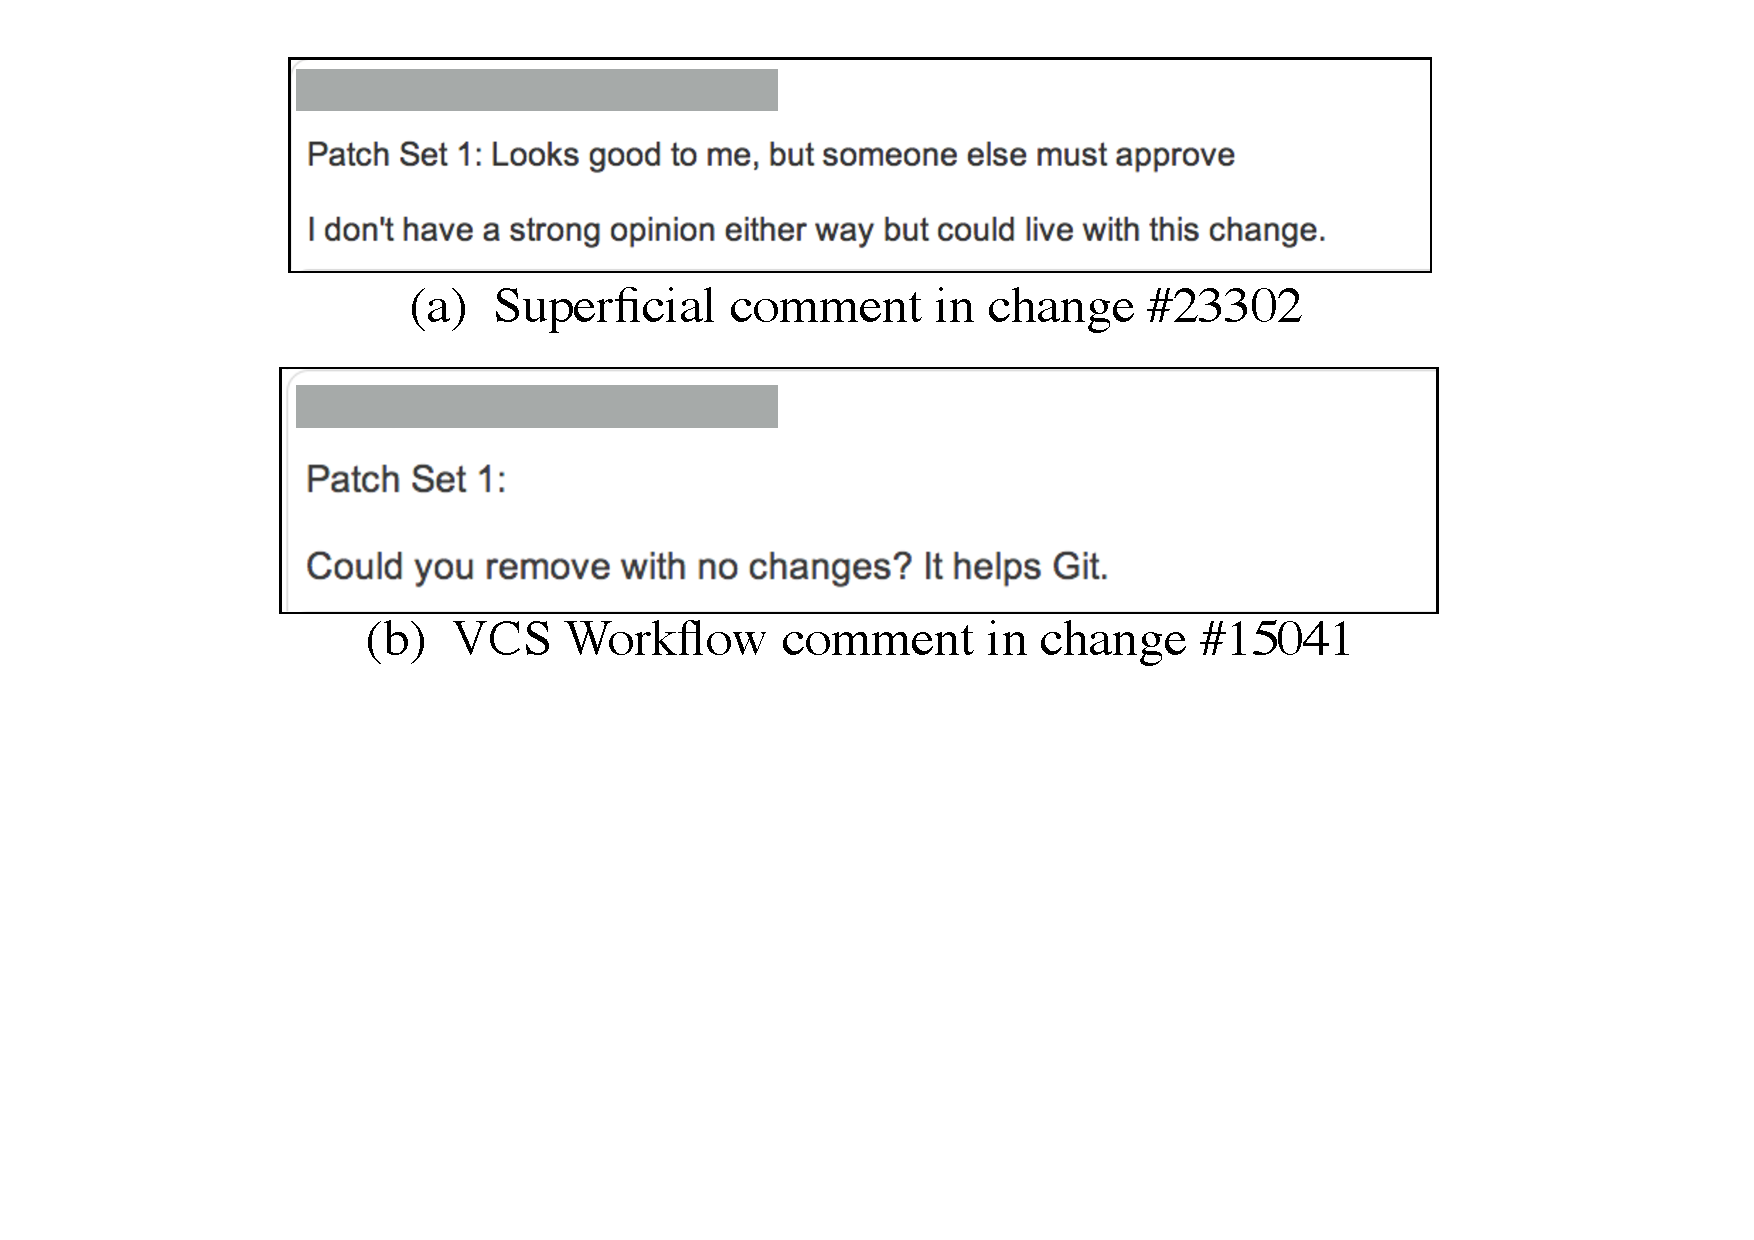
\includegraphics[scale=0.4, trim= 100 250 0 0, clip=true]{comment_examples}
\caption{Examples of comment in code reviews of Qt project.}
\label{fig:example}
\end{figure}

